\documentclass[11pt]{article}

\usepackage[T1]{fontenc}
\usepackage[margin=1in]{geometry}
\usepackage{booktabs}
\usepackage{enumitem}
\usepackage{graphicx}
\usepackage{tabularx}
\usepackage[hidelinks]{hyperref}
\usepackage{xurl}

\graphicspath{{docs/figures/}{figures/}}

\hypersetup{
  pdftitle={Projected Daily Fire Weather Index Methodology},
  pdfauthor={Degree Day}
}

\setlist{nosep,leftmargin=*}
\setlength{\parindent}{0pt}
\setlength{\parskip}{0.6em}

\title{Projected Daily Fire Weather Index Methodology}
\author{Degree Day}
\date{September 2026}

\begin{document}
\maketitle

\section{Overview}

The purpose of this workflow is to estimate how daily fire-weather conditions
may change under future climate scenarios. Its principal outputs are daily
fields of the Canadian Forest Fire Weather Index System (CFFWIS), including the
Fire Weather Index (FWI) and its five component indices, together with annual
summary indicators derived from those daily fields.

Daily FWI cannot be calculated reliably from annual or monthly climate
projections. It is a sequential index system: today's moisture codes depend on
the preceding weather and on the previous day's state. The calculation therefore
requires a continuous daily record of temperature, relative humidity,
precipitation, and wind speed. Errors in any of these inputs can accumulate or
interact nonlinearly in the resulting fire-weather indices.

Raw global climate-model output is not suitable for direct local FWI
calculation. Models have systematic biases in the distributions and seasonality
of the required variables, use different grids and calendars, and resolve the
atmosphere at a much coarser scale than is useful for local fire-weather
assessment. In particular, precipitation occurrence and intensity, near-surface
humidity, wind, and temperature extremes can differ materially from the
historical climate represented by reanalysis data.

The workflow addresses these limitations by placing all models on a common
daily $1^{\circ}$ grid, adjusting their historical distributions against a
reanalysis reference while retaining simulated climate-change signals, and
statistically downscaling the adjusted fields to $0.1^{\circ}$. Quality control
is applied throughout before the daily CFFWIS indices are calculated with
xclim. The result is a consistent set of historical and scenario-based future
daily FWI estimates designed for comparing changes across places, years,
models, and emissions pathways.

The production workflow processes four variables:
\begin{itemize}
  \item near-surface air temperature (\texttt{tas});
  \item near-surface relative humidity (\texttt{hurs});
  \item precipitation (\texttt{pr}); and
  \item near-surface wind speed (\texttt{sfcWind}).
\end{itemize}
These are the meteorological inputs required to calculate the Canadian Forest
Fire Weather Index System (CFFWIS). Other variables, including
\texttt{prsnratio}, are not downscaled in this production workflow.

\section{Climate-model selection}

The ensemble uses the five primary climate models selected for ISIMIP3b.
ISIMIP selected these models based on data availability, historical
performance, process representation, structural independence, and climate
sensitivity \cite{lange2021,frieler2026}. Together they include lower- and
higher-sensitivity models and therefore sample a broad range of possible
climate responses.

\begin{figure}[htbp]
\centering
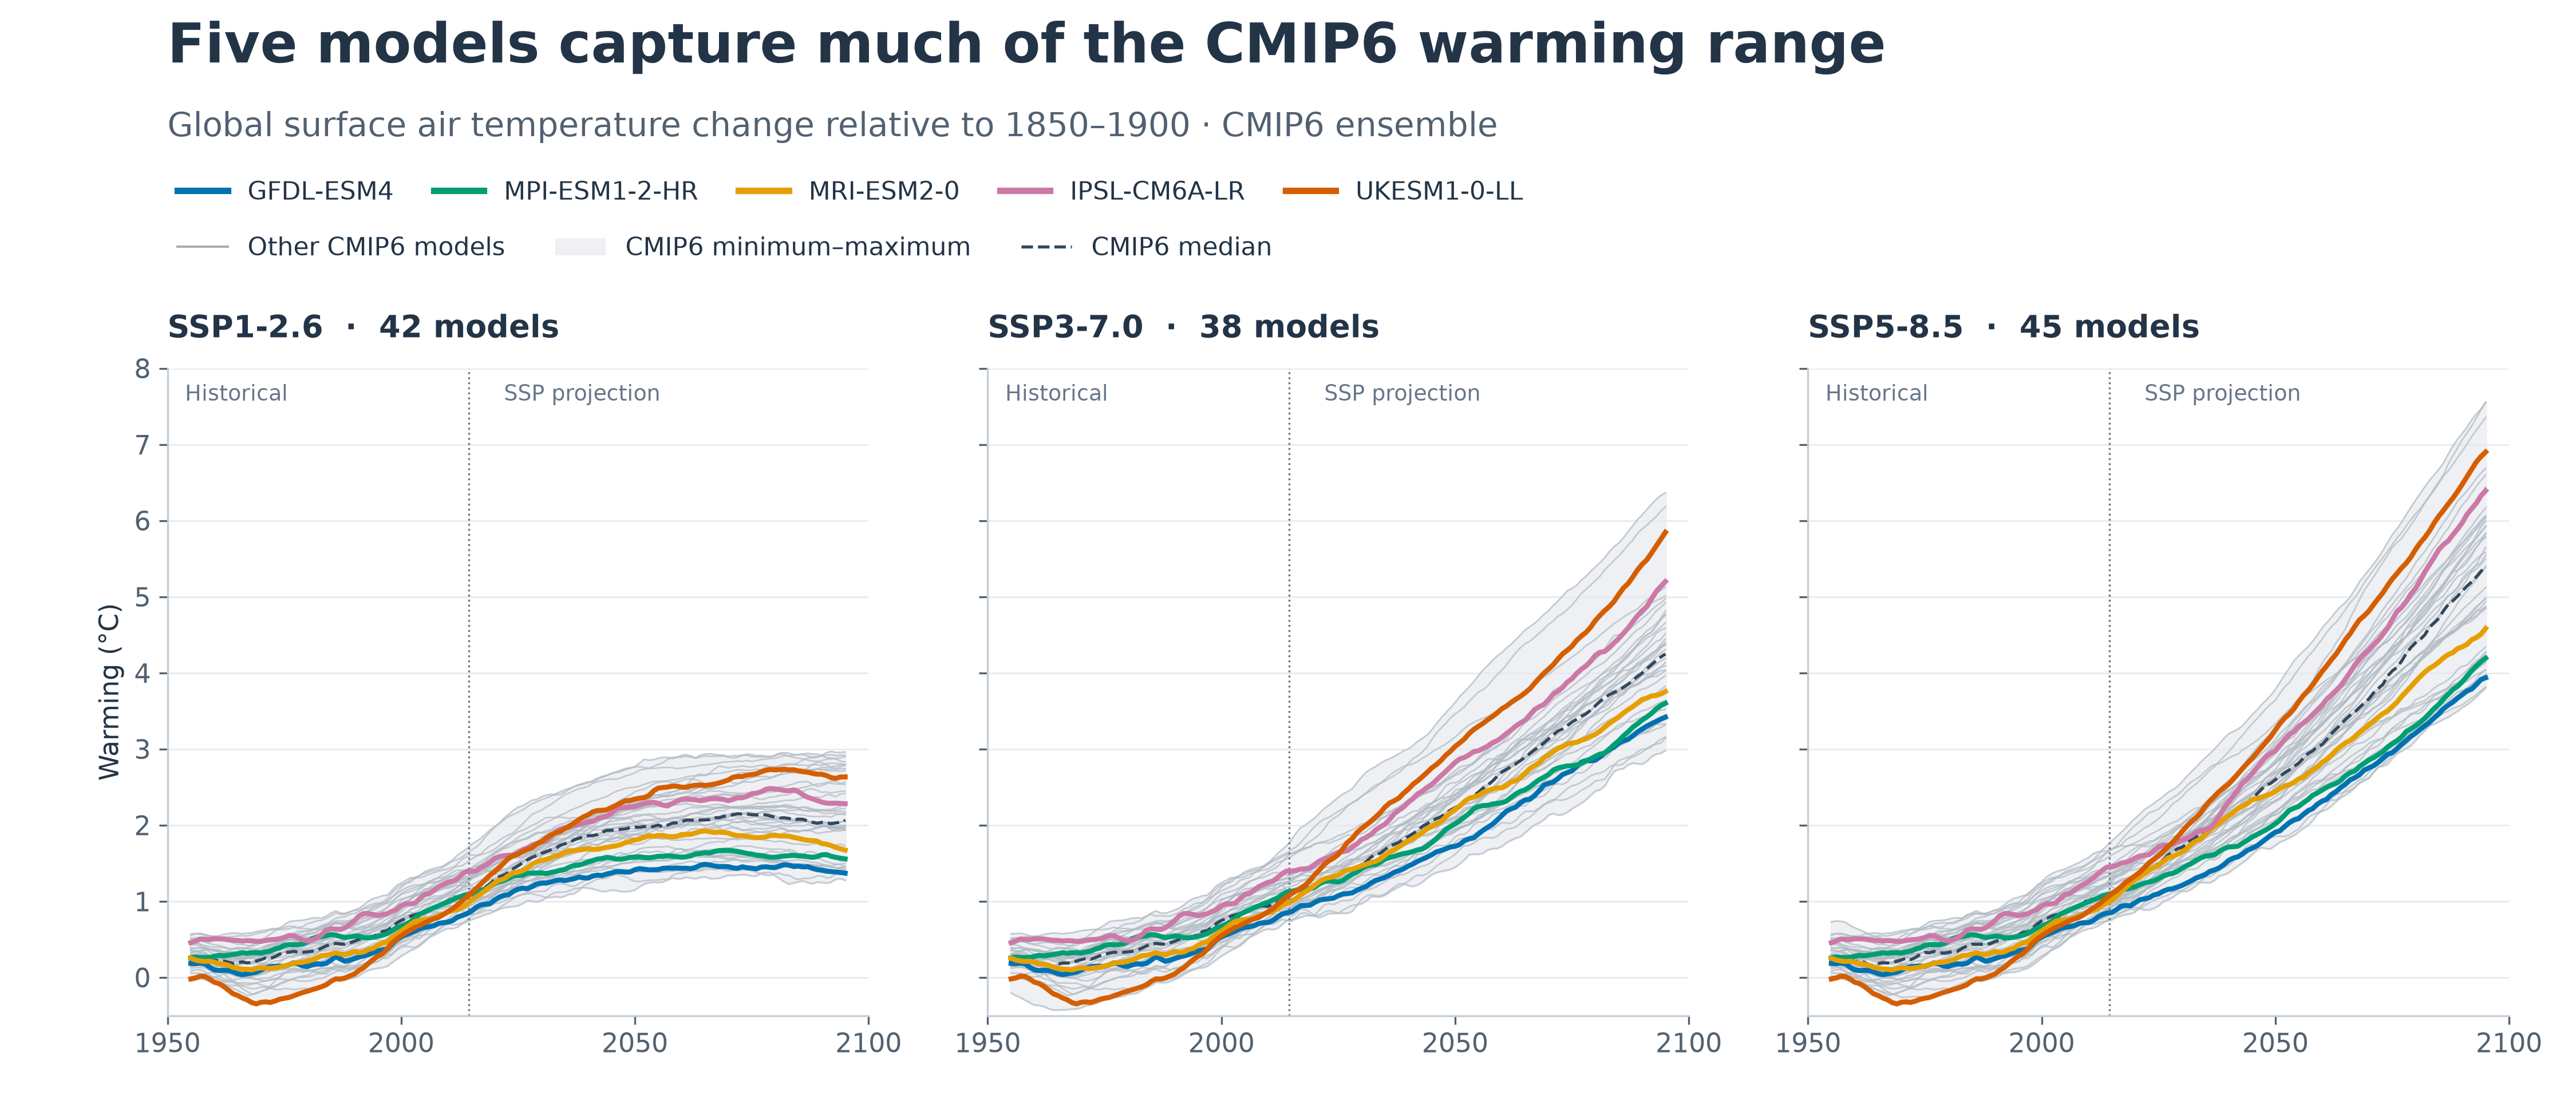
\includegraphics[width=\textwidth]{cmip6_model_range.png}
\caption{Global temperature trajectories illustrating how the five selected
models sample much of the broader CMIP6 warming range under lower-, medium-,
and high-forcing pathways. The highlighted models are intended to represent
climate-response diversity rather than a probability distribution.}
\label{fig:model-range}
\end{figure}

\begin{table}[htbp]
\centering
\caption{Selected models and projection pathways currently available in the
Sailfish archive. A dash indicates that the pathway is not currently present.}
\label{tab:model-scenarios}
\small
\begin{tabular}{lccccc}
\toprule
Model & Sensitivity & SSP1-2.6 & SSP2-4.5 & SSP3-7.0 & SSP5-8.5 \\
\midrule
GFDL-ESM4     & Lower  & Yes & Yes & Yes & Yes \\
MPI-ESM1-2-HR & Lower  & Yes & Yes & Yes & Yes \\
MRI-ESM2-0    & Lower  & Yes & Yes & Yes & Yes \\
IPSL-CM6A-LR  & Higher & Yes & Yes & --  & --  \\
UKESM1-0-LL   & Higher & Yes & Yes & --  & --  \\
\bottomrule
\end{tabular}
\end{table}

The scenarios range from lower to very high future forcing, as summarized in
Table~\ref{tab:ssps}. SSP5-8.5 is treated as a high-end stress test, not as a
forecast or a ``business as usual'' scenario. CMIP6 and ScenarioMIP are
described by Eyring et al. \cite{eyring2016} and O'Neill et al.
\cite{oneill2016}.

\begin{table}[htbp]
\centering
\caption{SSP pathways represented in the project archive.}
\label{tab:ssps}
\small
\begin{tabularx}{\textwidth}{lXc}
\toprule
Pathway & Interpretation in this workflow & Models available \\
\midrule
SSP1-2.6 & Lower-forcing pathway & 5 of 5 \\
SSP2-4.5 & Intermediate-forcing pathway & 5 of 5 \\
SSP3-7.0 & Medium-high forcing with distinctive aerosol and land-use assumptions & 3 of 5 \\
SSP5-8.5 & Very-high-forcing pathway used as a high-end stress test & 3 of 5 \\
\bottomrule
\end{tabularx}
\end{table}

\section{Input standardization}

The raw model data are organized into two periods: historical (1989--2014) and
projection (2015--2100). Before bias adjustment, all four variables are
standardized to a regular global $1^{\circ}$ grid, a complete 365-day no-leap
calendar, consistent names and units, and physically valid ranges.

Temperature, humidity, and wind are interpolated to the common grid.
Precipitation is conservatively remapped to better preserve spatial totals.
Calendar conversion includes specific handling of leap days and 360-day model
calendars. Each standardized dataset is checked for complete dates, duplicate
or missing time steps, coordinate errors, unexpected dimensions, invalid
units, infinities, implausible values, and incomplete active time series.

\section{Reference data}

The observational reference covers 1993--2014 on nested $1^{\circ}$ and
$0.1^{\circ}$ grids. It is based primarily on ERA5-Land local-noon daily
weather \cite{munoz2021}.

Some mapped coastal land cells are not represented by native ERA5-Land. The
reference therefore applies a consistent ERA5-Land coastline repair and uses
supplementary regular ERA5 data where needed. Regular ERA5 is bilinearly
interpolated from $0.25^{\circ}$ to $0.1^{\circ}$ and is incorporated only
after available ERA5-Land data and the coastline repair \cite{hersbach2020}.

A common land-support mask is used for all four variables. The $0.1^{\circ}$
reference supplies the fine-scale spatial pattern, while an area-weighted
$1^{\circ}$ version supplies the training target for bias adjustment.

\begin{figure}[htbp]
\centering
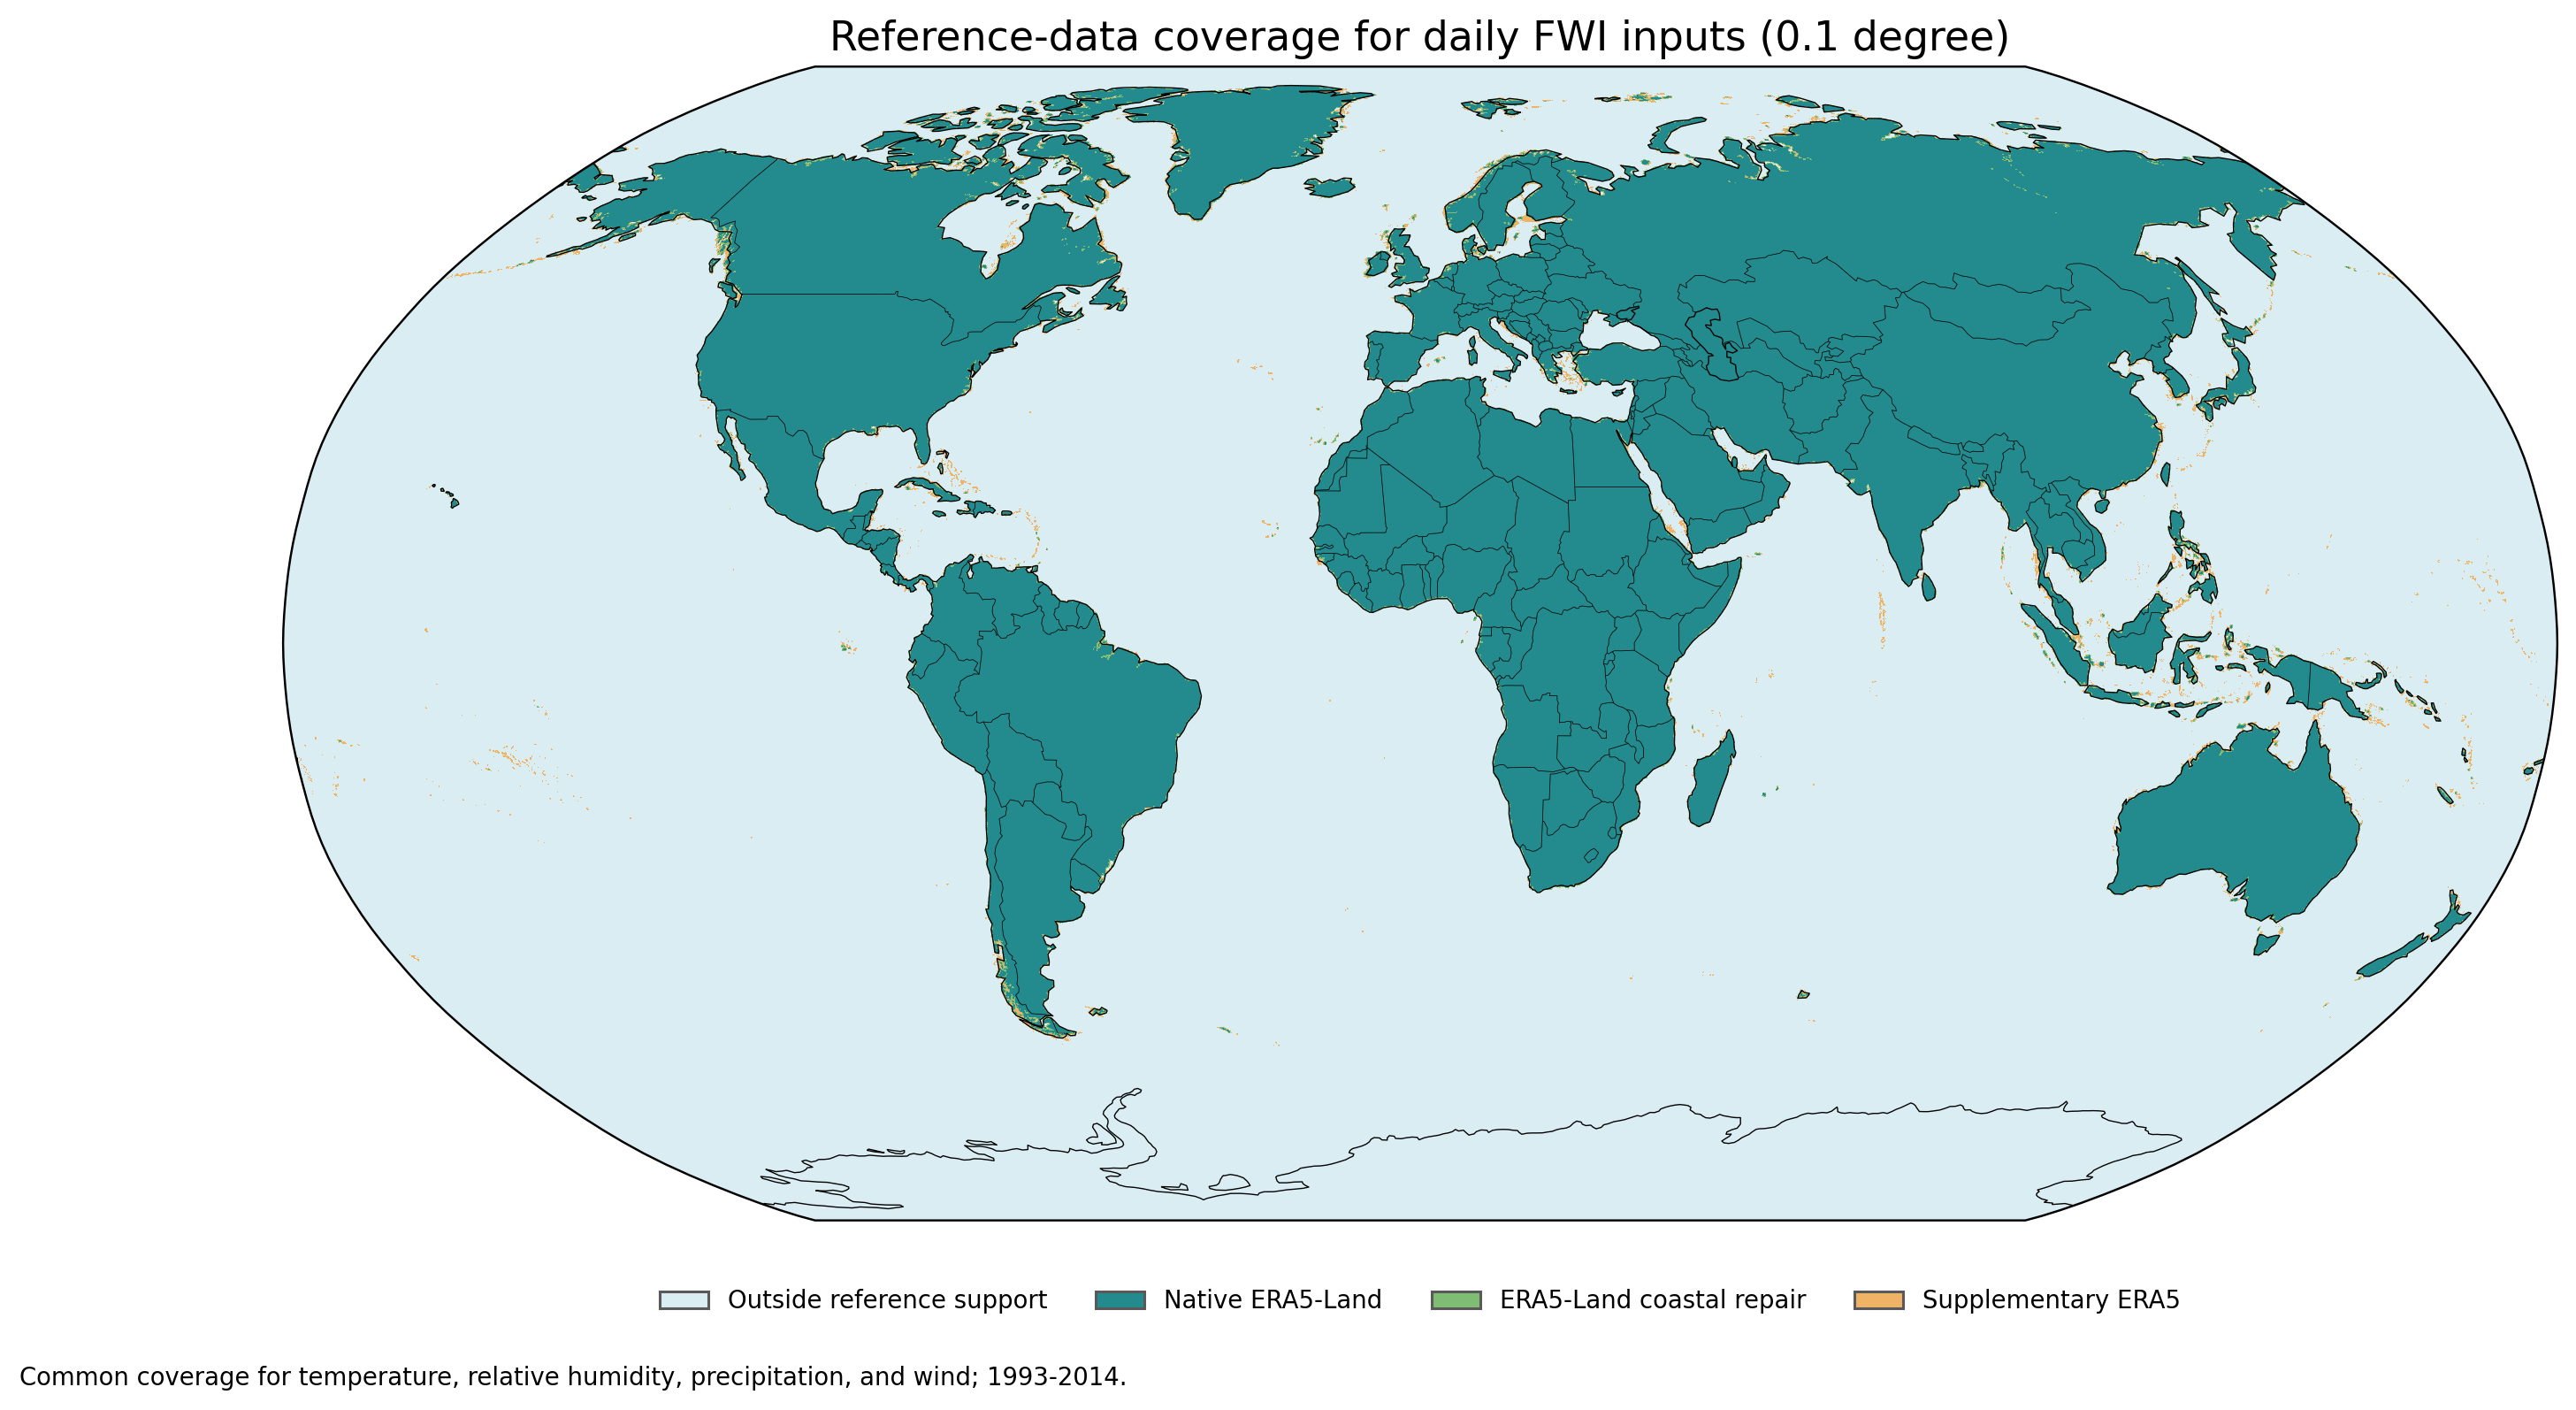
\includegraphics[width=\textwidth]{reference_source_coverage.png}
\caption{Coverage and source composition of the $0.1^{\circ}$ daily reference
used for temperature, relative humidity, precipitation, and wind speed. Native
ERA5-Land is retained wherever available; mapped coastal land is completed by
the common ERA5-Land repair and supplementary regular ERA5 data.}
\label{fig:reference-coverage}
\end{figure}

This differs from official ISIMIP3b, which used W5E5 at $0.5^{\circ}$
resolution. The official configuration is documented by Lange
\cite{lange2021}.

\section{Bias adjustment}

Bias adjustment is trained independently for each model, variable, and
$1^{\circ}$ grid cell using the overlap between the historical model data and
the 1993--2014 reference. The workflow uses trend-aware methods from xsdba:
\begin{itemize}
  \item temperature uses additive detrended quantile mapping;
  \item relative humidity uses bounded quantile-delta mapping;
  \item precipitation uses multiplicative quantile-delta mapping with explicit
        treatment of dry days; and
  \item wind speed uses multiplicative quantile-delta mapping.
\end{itemize}

The QDM approach follows Cannon et al. \cite{cannon2015}. Conventional quantile
mapping can alter a model's projected trends, particularly in precipitation
extremes. QDM instead adjusts the historical distribution toward the reference
while explicitly preserving the model-projected change at corresponding
quantiles. A moving seasonal window represents the annual cycle without
introducing abrupt month-boundary transitions.

The adjustment is univariate: each weather variable is treated separately.
The inter-variable MBCn bias-adjustment stage is not used. ISIMIP3b also
omitted that optional stage after it produced overfitting and spatial-coherence
problems \cite{lange2021}. Trained relationships can be cached and reused for
historical and future periods without changing the resulting values.

\section{Spatial downscaling}

After bias adjustment, each $1^{\circ}$ field is downscaled separately to the
$0.1^{\circ}$ reference grid using MBCnSD. At a high level, the method:
\begin{enumerate}
  \item interpolates the adjusted model field to the fine grid;
  \item learns the historical distribution among fine cells within each
        coarse parent cell;
  \item adjusts the fine-grid values toward that spatial distribution; and
  \item preserves the area-weighted climate-model signal of the parent cell.
\end{enumerate}

MBCnSD is based on multivariate quantile mapping, but its vector components in
this application are fine spatial cells, not different weather variables
\cite{cannon2018,lange2019}. The calculation is divided into restartable
geographic tiles. Each tile reads surrounding spatial context before
calculation, preventing processing-region boundaries from creating artificial
edges.

A $0.1^{\circ}$ output grid does not mean that the GCM dynamically resolves
climate at $0.1^{\circ}$. Fine-scale patterns are statistically inferred from
the historical reference, while the future signal still comes from the
coarser model. Some $1^{\circ}$ parent-cell structure can remain, particularly
in daily precipitation and derived FWI fields.

\begin{figure}[htbp]
\centering
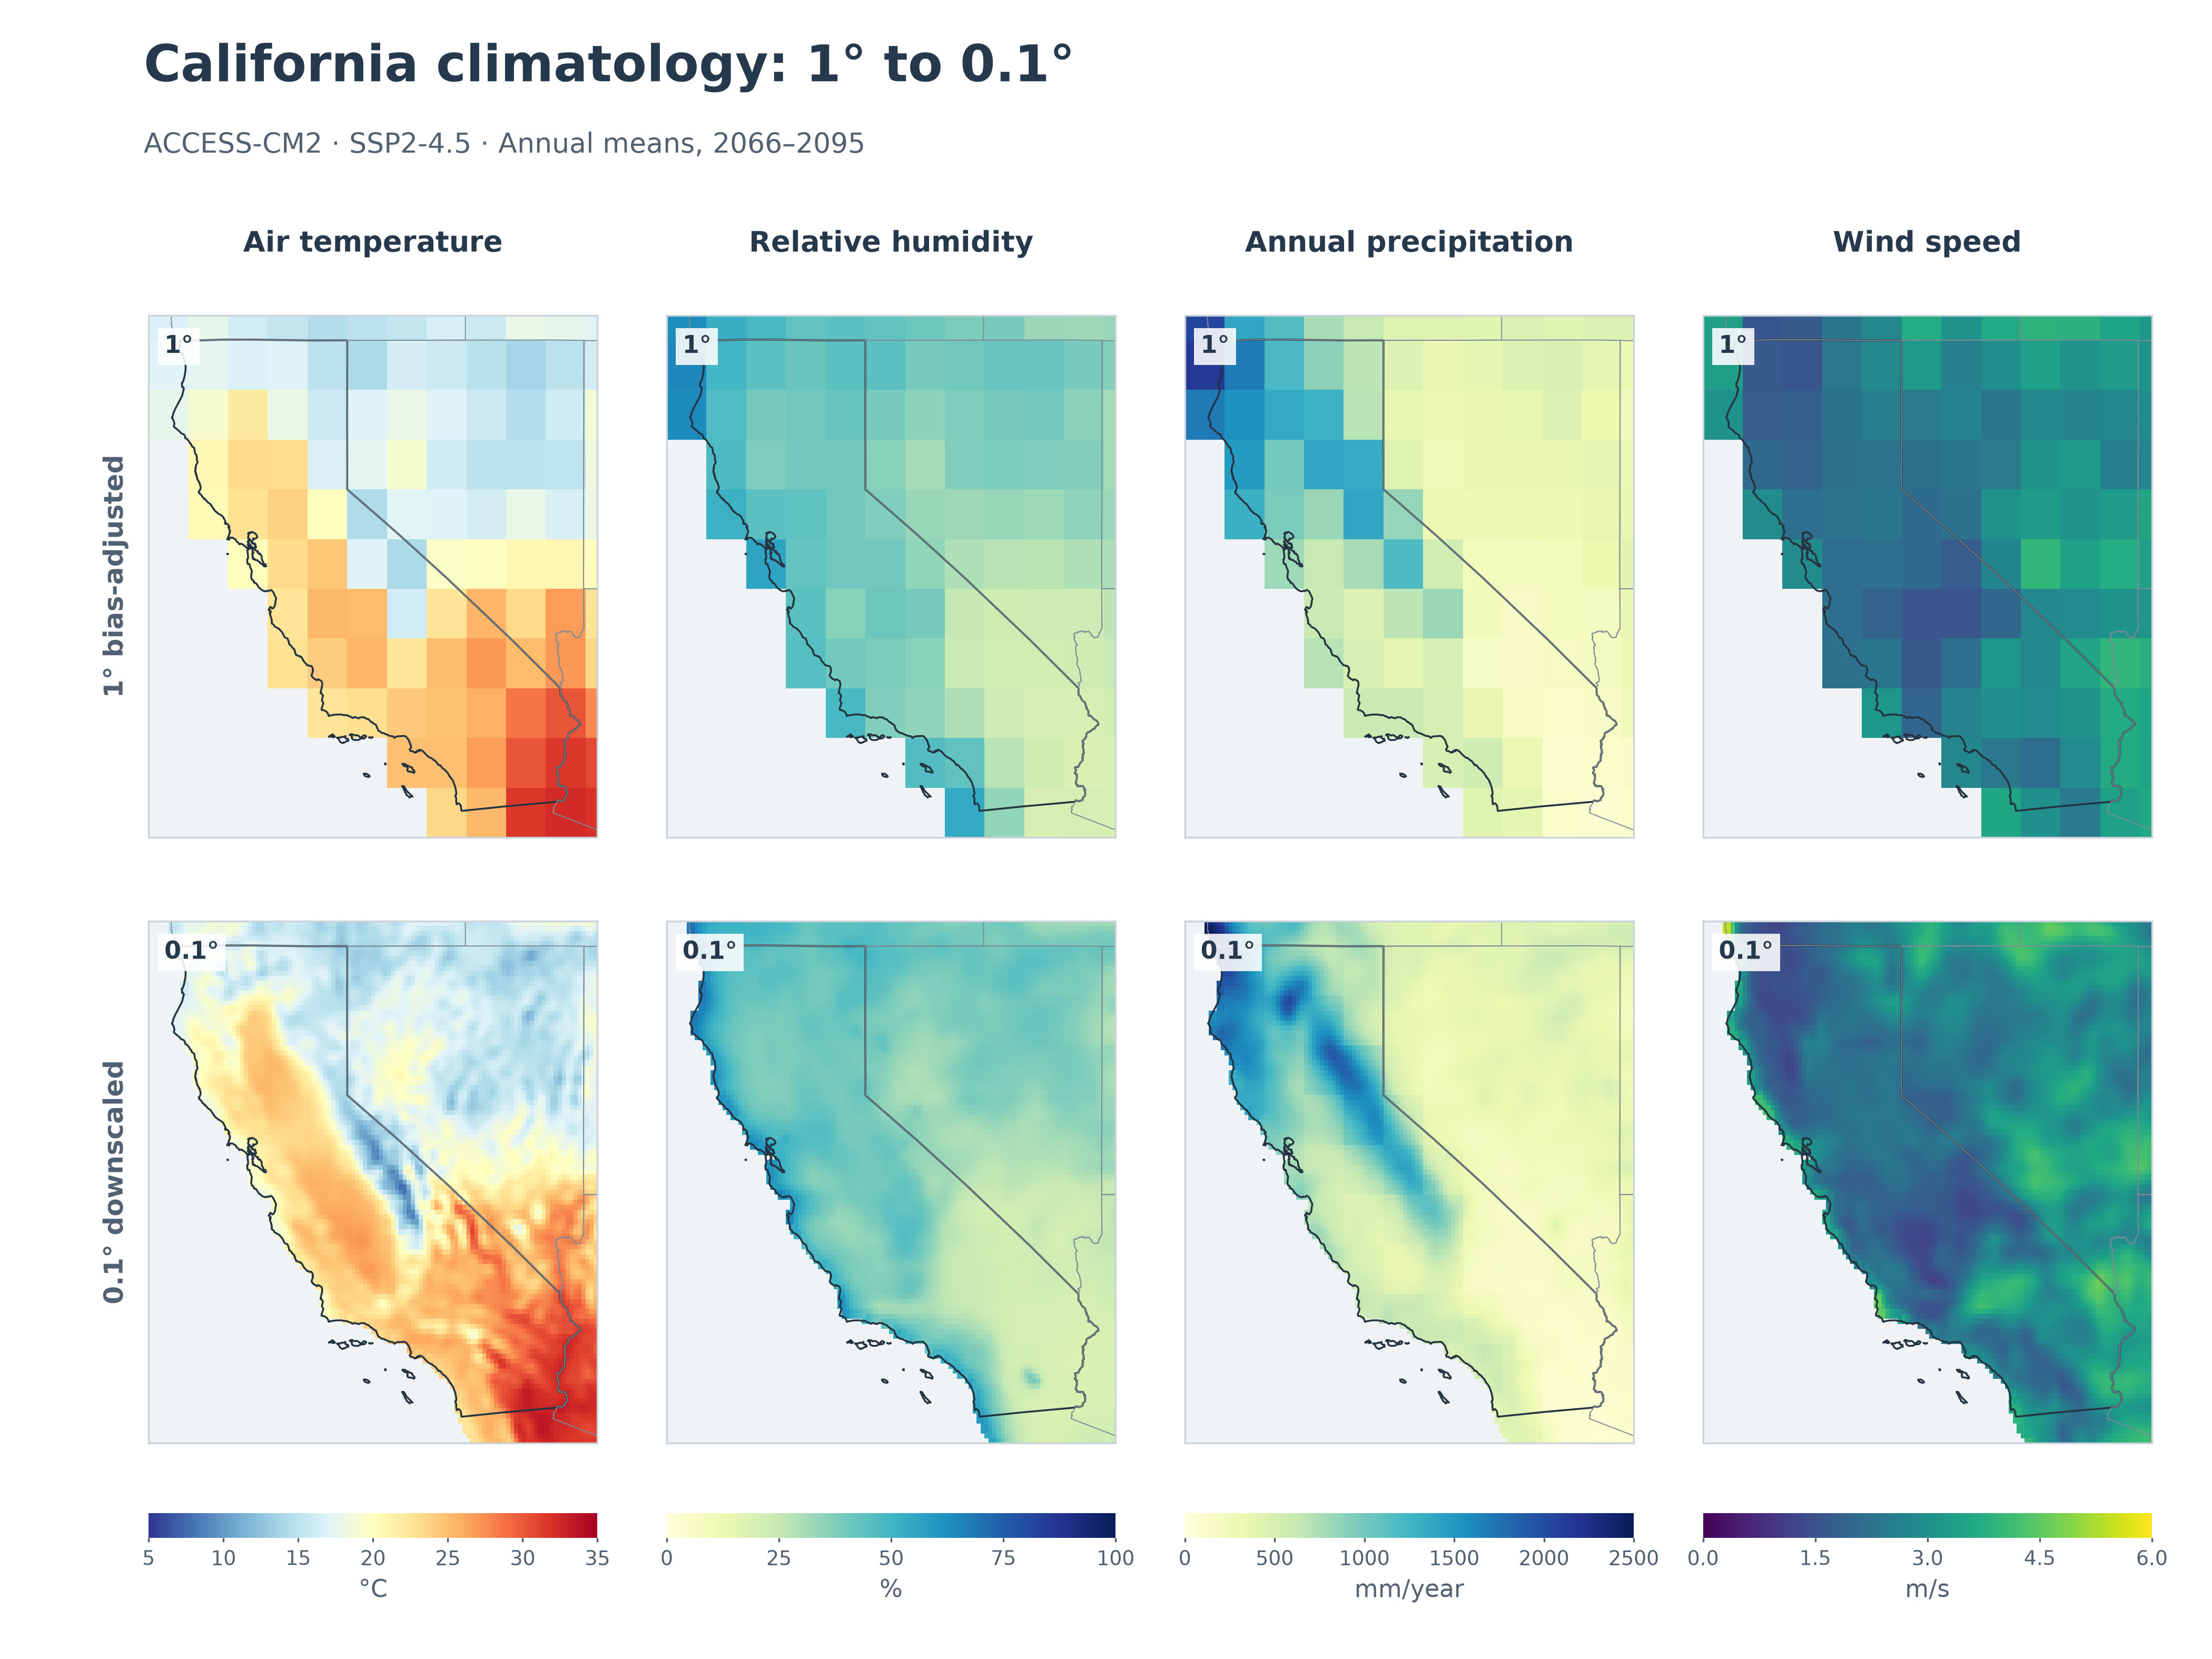
\includegraphics[width=\textwidth,height=0.66\textheight,keepaspectratio]
  {climate_downscaling_california.png}
\caption{Illustrative California climatologies before and after spatial
downscaling from $1^{\circ}$ to $0.1^{\circ}$ for ACCESS-CM2 under SSP2-4.5,
averaged over 2066--2095. The finer fields recover reference-scale spatial
patterns while retaining the climate-model signal at the coarser scale.}
\label{fig:california-downscaling}
\end{figure}

\section{Quality control and storage}

Quality control is performed at every major stage. It checks chronology,
calendar and coordinates, common coverage among variables, physical ranges,
missing supported land cells, spatial discontinuities, preservation of the
adjusted $1^{\circ}$ signal, and numerical accuracy after storage.

Global maps and regional views are inspected in addition to machine-readable
tests. This helps distinguish processing-tile seams from spatial structure
inherited from the parent climate-model grid. Extreme precipitation is capped
at 3,000~mm~day$^{-1}$, following a control used by the Climate Impact Lab
downscaleCMIP6 workflow \cite{cil2024}.

Final daily products are stored as compressed, scaled \texttt{int16} Zarr
datasets. Scale factors and offsets permit transparent decoding to physical
values. A reserved integer code distinguishes missing data from valid zeroes.

\section{Canadian Forest Fire Weather Index System}

All six daily CFFWIS components are calculated with xclim's
\nolinkurl{xclim.indices.fire.cffwis_indices} routine \cite{xclim2023}. The workflow does not
reimplement the Canadian FWI equations. It supplies the downscaled inputs,
maintains the calculation through time, applies the common land mask, and
validates and stores the outputs.

The daily outputs are the Fine Fuel Moisture Code (\texttt{ffmc}), Duff
Moisture Code (\texttt{dmc}), Drought Code (\texttt{dc}), Initial Spread Index
(\texttt{isi}), Build Up Index (\texttt{bui}), and Fire Weather Index
(\texttt{fwi}). The calculation uses temperature, relative humidity,
precipitation, wind speed, and latitude. It includes a temperature-defined fire
season and Drought Code overwintering. The system is described by Van Wagner
\cite{vanwagner1987}.

\subsection{Spin-up, boundary continuity, and restarts}

CFFWIS is stateful: the moisture codes on one day depend on their values on the
preceding day. At the beginning of a calculation, xclim applies the standard
start-up values of 85 for FFMC, 6 for DMC, and 15 for DC. The WF93 season method
then identifies seasonal start-up and shutdown, and DC overwintering carries
information from one fire season into the next.

The historical calculation begins on 1 January 1989. No separate historical
spin-up file is published. The years before the 1995--2014 reference interval
provide six complete years of model weather and CFFWIS evolution before the
historical thresholds and summary statistics are evaluated. This reduces
sensitivity of the reported reference-period indicators to the initial values,
although the earliest daily historical output should still be regarded as
initialization-affected.

For each model--scenario pathway, the projection calculation prepends the
1989--2014 historical meteorology before calling xclim. CFFWIS state therefore
evolves continuously across 31 December 2014 and 1 January 2015, including in
the Southern Hemisphere and other locations where the fire season may be active
at the archive boundary. Only the 2015--2100 portion is written to the
projection store. This preserves the convenient historical and projection
archive layout without reinitializing FFMC, DMC, DC, fire-season state, or DC
overwintering at the boundary.

Computational restart files serve a different purpose. The global calculation
is divided into spatial tiles, and a versioned success marker is written only after all
six indices for a tile have been stored and checked. A completed tile is skipped
when a job restarts; an interrupted tile is recomputed over its full requested
time interval. These markers are workflow checkpoints, not saved FFMC, DMC, DC,
season, or overwintering states. The implementation does not resume a tile from
an intermediate date. The checkpoint version changes when continuity semantics
change, preventing outputs made with an older initialization scheme from being
silently accepted.

Four annual indicators are derived from the daily xclim output:
\begin{description}[style=nextline]
  \item[\texttt{fwixx}] annual maximum FWI;
  \item[\texttt{fwixd}] annual count of days above the local historical
        95th-percentile FWI threshold;
  \item[\texttt{fwils}] annual count of days above the local historical FWI
        midrange; and
  \item[\texttt{fwisa}] annual maximum 90-day mean FWI.
\end{description}
The local thresholds are calculated from 1995--2014 and then held constant for
historical and future years. These indicators follow the concepts used by
Abatzoglou et al. \cite{abatzoglou2019}.

FWI describes weather conditions associated with potential fire behaviour. It
does not predict ignition, burned area, structure loss, smoke, or suppression
difficulty. Those outcomes also depend on fuels, vegetation, land management,
topography, human activity, and exposure.

\begin{figure}[htbp]
\centering
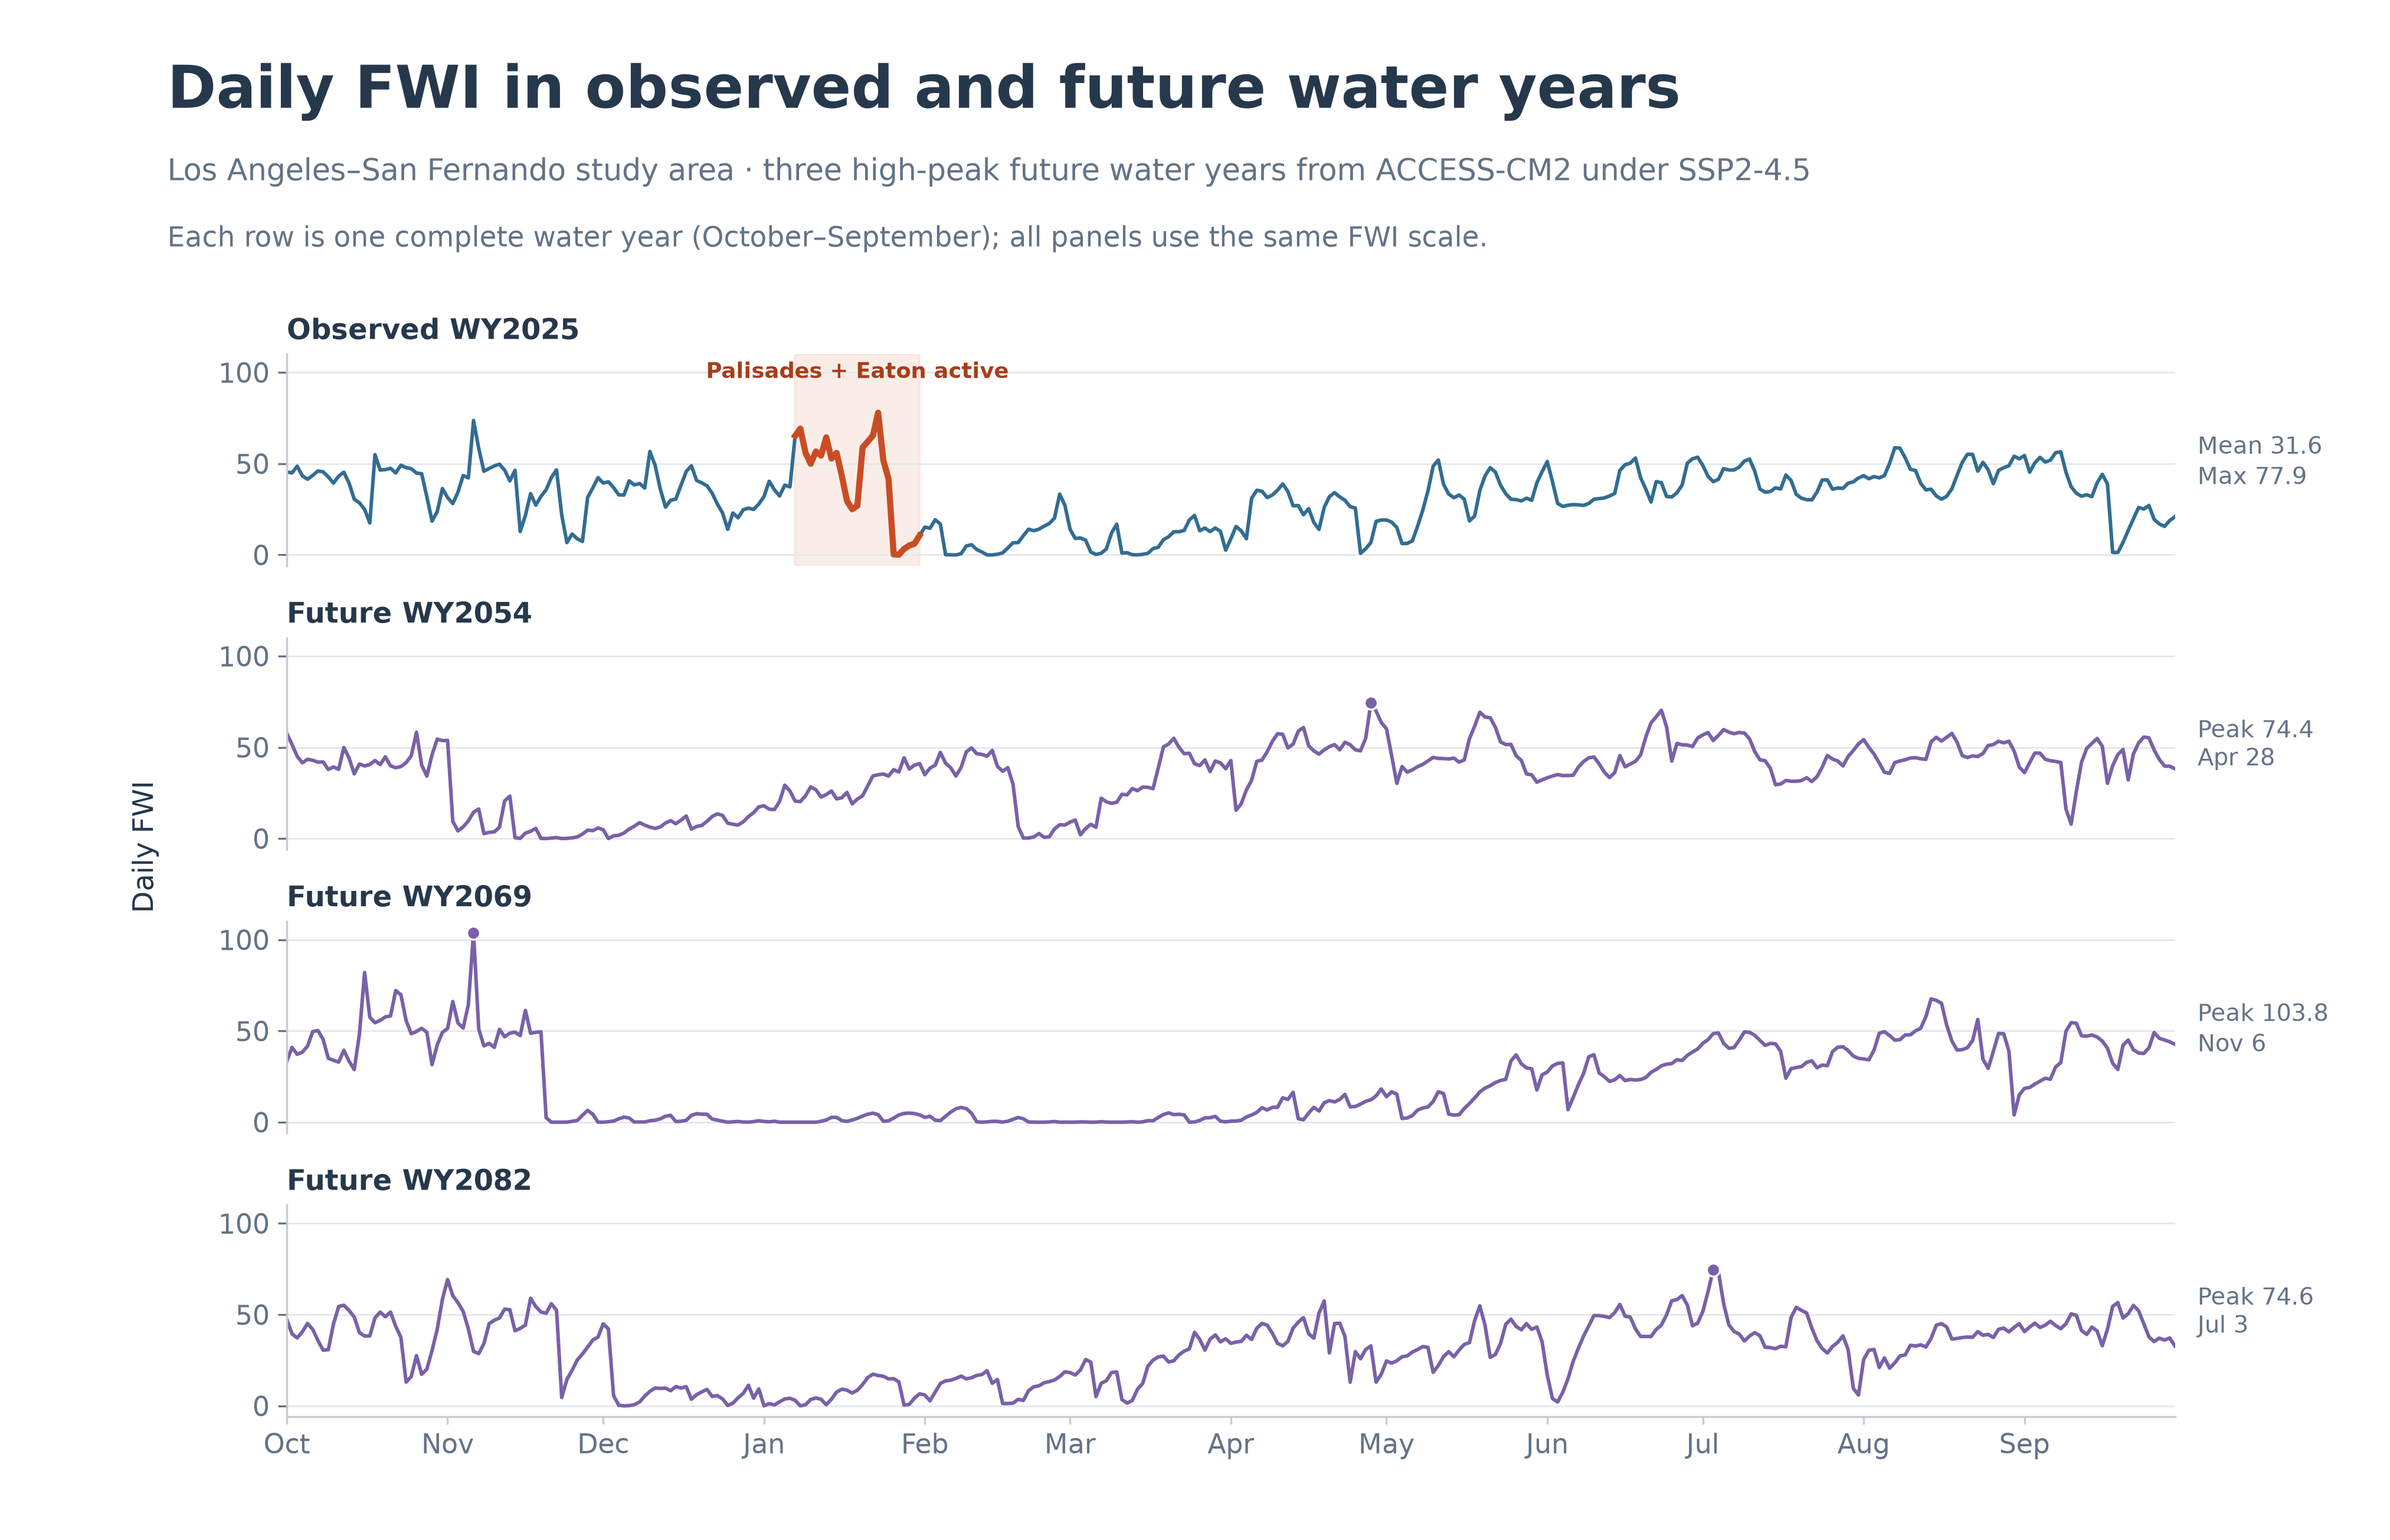
\includegraphics[width=\textwidth,height=0.63\textheight,keepaspectratio]
  {future_daily_fwi_peaks.png}
\caption{Example daily FWI sequences for the Los Angeles--San Fernando study
area. The observed 2025 water year is shown alongside three ACCESS-CM2
SSP2-4.5 water years selected for high seasonal peaks. Individual future years
are scenario realizations used to examine plausible daily conditions; they are
not forecasts for those calendar years.}
\label{fig:future-fwi-peaks}
\end{figure}

\section{Interpretation and limitations}

The product is based on climate scenarios rather than forecasts. Statistical
adjustment cannot correct errors in the model's underlying climate response,
and the fine-scale relationships observed during 1993--2014 are assumed to
remain applicable in future climates. The four variables are adjusted
independently, and the $0.1^{\circ}$ grid contains statistically inferred
detail rather than new high-resolution climate physics.

Reference uncertainty and the differing time semantics of supplementary
regular ERA5 data affect some coastal locations. Model and scenario uncertainty
must therefore be retained in downstream analysis. Results should be reported
across models and scenarios rather than as a single deterministic future.
The approach draws on ISIMIP3BASD methods, but the resulting dataset is not an
official ISIMIP3b forcing product or a bit-for-bit reproduction of the archived
ISIMIP3BASD software \cite{lange2022}.
Source-model licenses, institutional credits, software versions,
reference-data citations, and processing provenance must accompany published
or redistributed products.

\begin{thebibliography}{99}

\bibitem{abatzoglou2019}
Abatzoglou, J. T., Williams, A. P., and Barbero, R. (2019).
Global emergence of anthropogenic climate change in fire weather indices.
\emph{Geophysical Research Letters}, 46, 326--336.
\url{https://doi.org/10.1029/2018GL080959}.

\bibitem{xclim2023}
Bourgault, P., et al. (2023).
xclim: xarray-based climate data analytics.
\emph{Journal of Open Source Software}, 8, 5415.
\url{https://doi.org/10.21105/joss.05415}.

\bibitem{cannon2015}
Cannon, A. J., Sobie, S. R., and Murdock, T. Q. (2015).
Bias correction of GCM precipitation by quantile mapping: How well do methods
preserve changes in quantiles and extremes? \emph{Journal of Climate}, 28,
6938--6959.
\url{https://doi.org/10.1175/JCLI-D-14-00754.1}.

\bibitem{cannon2018}
Cannon, A. J. (2018).
Multivariate quantile mapping bias correction: an N-dimensional probability
density function transform for climate model simulations of multiple
variables. \emph{Climate Dynamics}, 50, 31--49.
\url{https://doi.org/10.1007/s00382-017-3580-6}.

\bibitem{eyring2016}
Eyring, V., et al. (2016).
Overview of the Coupled Model Intercomparison Project Phase 6 experimental
design and organization. \emph{Geoscientific Model Development}, 9,
1937--1958. \url{https://doi.org/10.5194/gmd-9-1937-2016}.

\bibitem{frieler2026}
Frieler, K., et al. (2026).
Scenario set-up and the new CMIP6-based climate-related forcings provided
within ISIMIP3b. \emph{Geoscientific Model Development}, 19, 4095--4146.
\url{https://doi.org/10.5194/gmd-19-4095-2026}.

\bibitem{hersbach2020}
Hersbach, H., et al. (2020).
The ERA5 global reanalysis. \emph{Quarterly Journal of the Royal Meteorological
Society}, 146, 1999--2049. \url{https://doi.org/10.1002/qj.3803}.

\bibitem{lange2019}
Lange, S. (2019).
Trend-preserving bias adjustment and statistical downscaling with
ISIMIP3BASD. \emph{Geoscientific Model Development}, 12, 3055--3070.
\url{https://doi.org/10.5194/gmd-12-3055-2019}.

\bibitem{lange2021}
Lange, S. (2021).
ISIMIP3b bias adjustment fact sheet.
\url{https://www.isimip.org/documents/413/ISIMIP3b_bias_adjustment_fact_sheet_Gnsz7CO.pdf}.

\bibitem{lange2022}
Lange, S. (2022).
ISIMIP3BASD v3.0.2 source archive.
\url{https://zenodo.org/records/7151476}.

\bibitem{munoz2021}
Munoz-Sabater, J., et al. (2021).
ERA5-Land: a state-of-the-art global reanalysis dataset for land applications.
\emph{Earth System Science Data}, 13, 4349--4383.
\url{https://doi.org/10.5194/essd-13-4349-2021}.

\bibitem{oneill2016}
O'Neill, B. C., et al. (2016).
The Scenario Model Intercomparison Project for CMIP6.
\emph{Geoscientific Model Development}, 9, 3461--3482.
\url{https://doi.org/10.5194/gmd-9-3461-2016}.

\bibitem{vanwagner1987}
Van Wagner, C. E. (1987).
\emph{Development and Structure of the Canadian Forest Fire Weather Index
System}. Canadian Forestry Service, Forestry Technical Report 35.
\url{https://www.canadawildfire.org/_files/ugd/90df79_f7ee78aa08b54e4a9b691a802dbb30c1.pdf}.

\bibitem{cil2024}
Climate Impact Lab (2024).
Global Downscaled Projections for Climate Impacts Research: downscaleCMIP6.
\url{https://github.com/ClimateImpactLab/downscaleCMIP6}.

\end{thebibliography}

\end{document}
